%!TEX program = xelatex
% 完整编译: xelatex -> biber/bibtex -> xelatex -> xelatex
\documentclass[lang=en,11pt,a4paper,bibend=bibtex]{elegantpaper}

\title{Finite element methods}
\author{Wenchong Huang}


% 本文档命令
\usepackage{array}
\usepackage{float}
\usepackage{multirow}
\newcommand{\ccr}[1]{\makecell{{\color{#1}\rule{1cm}{1cm}}}}

\begin{document}

\maketitle

\section{Introduction}

In this month, my major work is learning the FEM.
In the theoretical aspect, I learned how to prove the convergence of 
linear elements in the $H^1$ and the $L^2$ norm. 
In the technical aspect, things I learned are listed below.

\begin{enumerate}
    \item Make the meshgrid.
    \item A solver to elliptic equations.
    \item The adaptive refinment technich.
    \item The multigrid technich.
    \item A solver to the heat equation.
    \item A solver to the advection-diffusion equation.
    \item A solver to the convection-diffusion equation.
    \item A solver to the INSE with UPPE.
\end{enumerate}

The codes are based on the deal.II liberary. 
I will choose some numerical tests to report in this article.


\section{The reports}

\subsection{The meshgrid}

I made a hexahedral meshgrid for our 3D ball-dragging problem.
The meshgrid could be successively refined.

\begin{figure}[H]
    \centering
    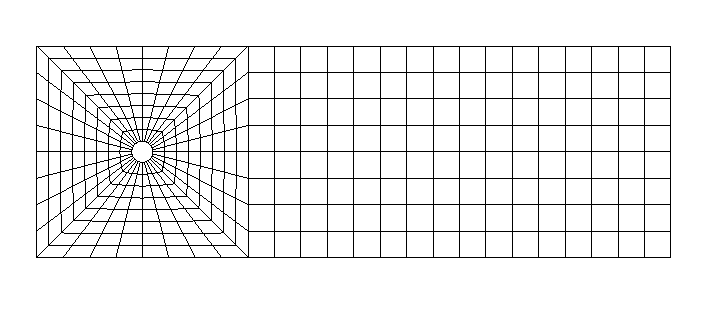
\includegraphics[width=0.7\textwidth]{png/level2_z=5.png}
    \caption{The snapshot of the meshgrid inside the plane $z=5$.}
\end{figure}

\subsection{The advection-diffusion equation}

Write the advection-diffusion equation as
\begin{equation}
    \frac{\partial \phi}{\partial t}=L(\phi,t)+D(\phi),
\end{equation}
where
\begin{equation*}
    L(\phi,t)=-\nabla\cdot(\mathbf{u}\phi)+f(\mathbf{x},t),
    \qquad D(\phi)=\nu\Delta\phi.
\end{equation*}

The time-discretization method is the IMEX-trapezoidal method:
\begin{align*}
    \left(1-\frac{k}{2}D\right)\phi^* &= 
    \phi^n+kL(\phi^n,t_n)+\frac{k}{2}D(\phi^n),\\
    \phi^{n+1} &= \phi^n 
    + \frac{k}{2}L(\phi^n,t_{n+1}) + \frac{k}{2}D(\phi^n)
    + \frac{k}{2}L(\phi^*,t_{n+1}) + \frac{k}{2}D(\phi^*).
\end{align*}

The space-discretization method is $Q_1$ elements. 
The test problem is \textbf{Gaussian Patch in Vortex Shear}, 
follows \cite{Zhang2012}, except the boundary conditions, 
which are modified to the homogeneous Dirichlet.

\begin{figure}[H]
    \centering
    \begin{minipage}[t]{0.45\linewidth}
        \centering
        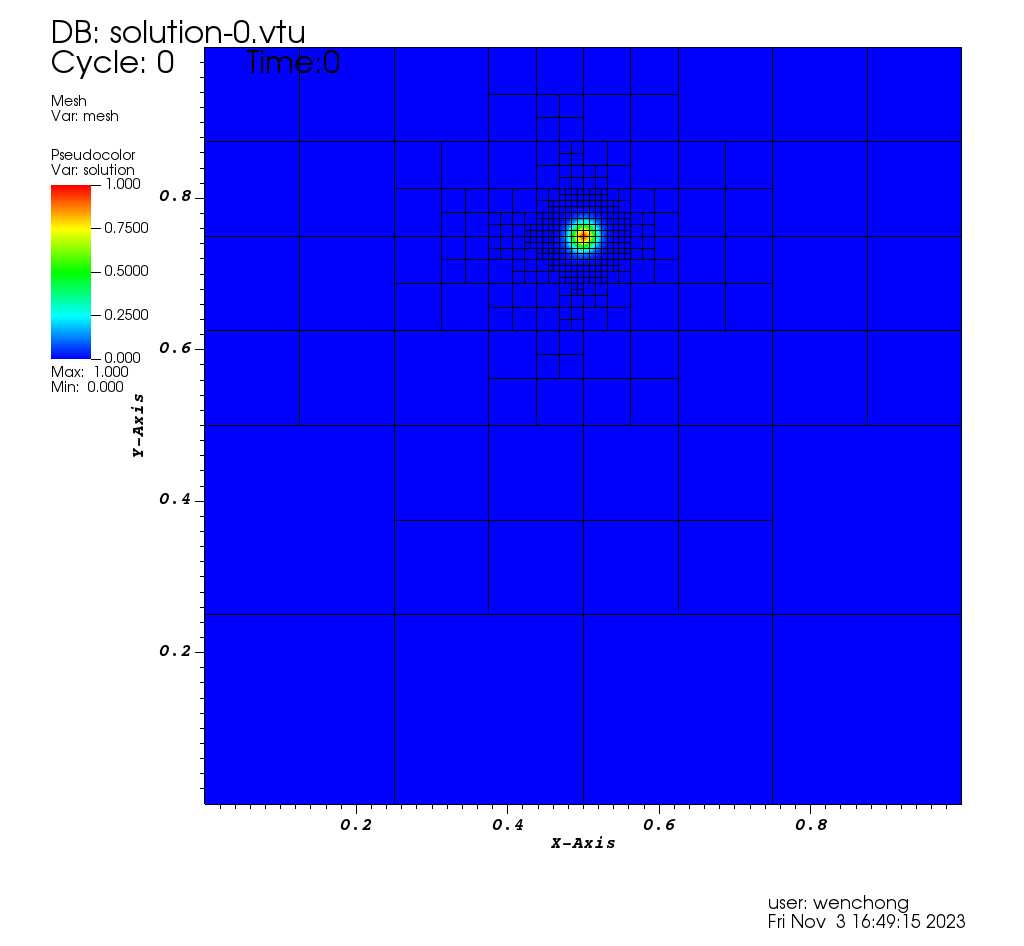
\includegraphics[width=0.9\linewidth]{png/adv-dif-0.png}
        \caption*{(a) $t=0$.}
    \end{minipage}
    \begin{minipage}[t]{0.45\linewidth}
        \centering
        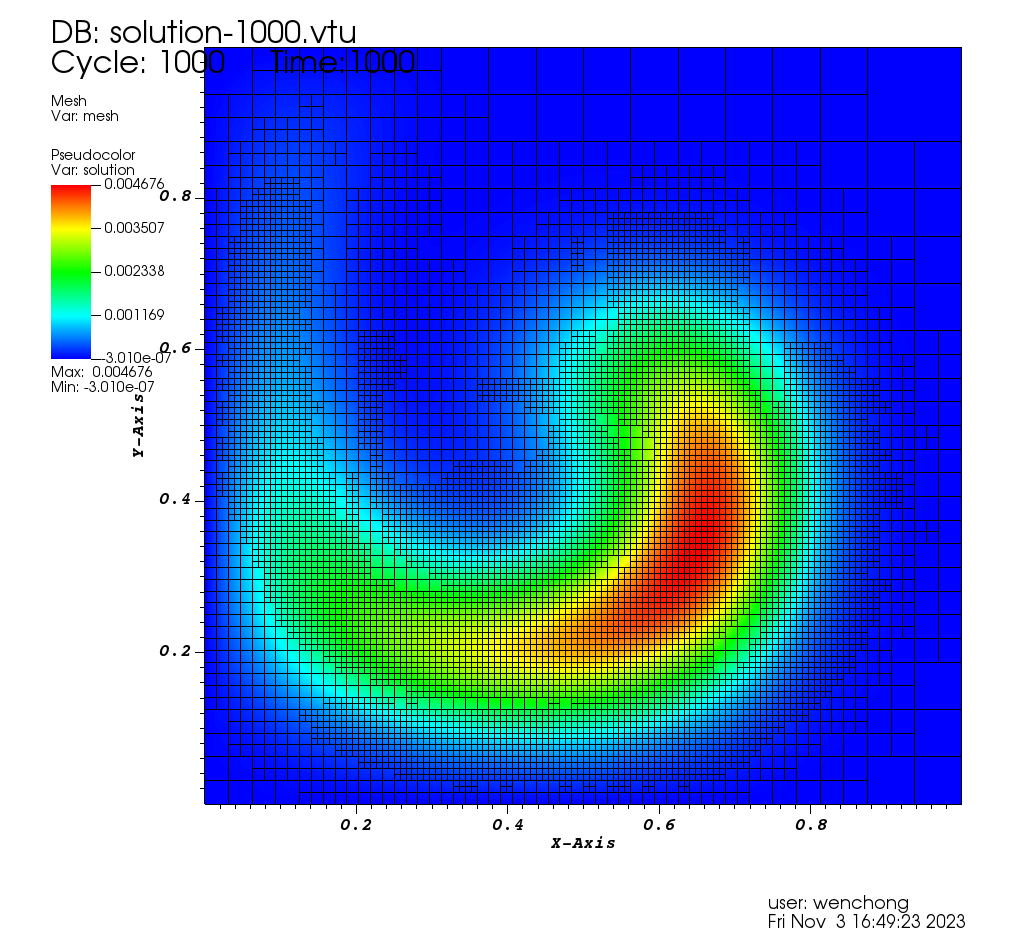
\includegraphics[width=0.9\linewidth]{png/adv-dif-1.png}
        \caption*{(b) $t=10$.}
    \end{minipage}
    \caption{Meshgrid and solution plots of the Gaussian Patch in 
    Vortex Shear test.}
\end{figure}

\subsection{The convection-diffusion equation}

Write the convection-diffusion equation as
\begin{equation}
    \frac{\partial \mathbf{u}}{\partial t}=L(\mathbf{u},t)+D(\mathbf{u}),
\end{equation}
where
\begin{equation*}
    L(\mathbf{u},t)=-(\mathbf{u}\cdot\nabla)\mathbf{u}
    +\mathbf{g}(\mathbf{x},t),
    \qquad D(\mathbf{u})=\nu\Delta\mathbf{u}.
\end{equation*}

Still, use the IMEX-trapezoidal method and $Q_1$ elements.
The test problem is \textbf{Vortex Shear}, follows \cite{Zhang2011}, 
is derived from the exact solution
\begin{equation}
    \mathbf{u}(x,y)=\cos\frac{\pi t}{T}(\sin^2(\pi x)\sin(2\pi y),
    -\sin(2\pi x)\sin^2(\pi y)),
\end{equation}
where $T=1$. To satisfy the CFL condition, we set the time-step
$k=\frac{h}{31.25}$. The numerical test showed the 2nd-order
convergence rate.

\begin{table}[H]
    \centering
    \begin{tabular}{cccccc}
    \hline
    $h$                                    & $\frac{1}{32}$ & 
    Rate & $\frac{1}{64}$ & Rate & $\frac{1}{128}$ \\ \hline
    $u_1$, $L_2$, $t=\frac{T}{2}$ & 2.11e-03    & 1.99 
    & 5.31e-04   & 2.01 & 1.32e-04    \\
    $u_2$, $L_2$, $t=\frac{T}{2}$ & 2.11e-03    & 1.99 
    & 5.31e-04   & 2.01 & 1.32e-04    \\ \hline
    $u_1$, $L_2$, $t=T$           & 9.25e-04   & 1.99 
    & 2.33e-04   & 2.02 & 5.76e-05    \\
    $u_2$, $L_2$, $t=T$           & 9.25e-04   & 1.99 
    & 2.33e-04   & 2.02 & 5.76e-05    \\ \hline
    \end{tabular}
    \caption{Solution errors and convergence of the Vortex Shear test.
     $\nu=0.01$.}
\end{table}

\subsection{The INSE}

Write the Navier-Stokes equation as
\begin{equation}
    \frac{\partial \mathbf{u}}{\partial t}=L(\mathbf{u},t)+D(\mathbf{u}),
\end{equation}
where
\begin{equation*}
    L(\mathbf{u},t)=-\nabla p-(\mathbf{u}\cdot\nabla)\mathbf{u}
    +\mathbf{f}(\mathbf{x},t),
    \qquad D(\mathbf{u})=\nu\Delta\mathbf{u},
\end{equation*}
with the Dirichlet boundary conditions
\begin{equation}
    \mathbf{u}=\mathbf{g}\quad \text{on}\;\partial\Omega.
\end{equation}

The pressure field $p$ should ensure that
\begin{equation}
    \nabla\cdot \mathbf{u}=0\quad \text{in}\;\Omega.
\end{equation}

We ues the IMEX-trapezoidal method and $Q_2$ elements. 
After we extrapolated $\mathbf{u}$, we update the pressure by 
the UPPE formulation, see \cite{Liu2010},
\begin{equation}
    \int_\Omega \nabla p \cdot \nabla \psi \;\text{d}\mathbf{x} = 
    \int_{\partial\Omega} (\nu(\nabla \times \mathbf{u}) \cdot 
    (\mathbf{n} \times \partial_t \mathbf{g}) \psi ) \;\text{d}A
    + \int_\Omega \mathbf{F} \cdot \nabla \psi \;\text{d}\mathbf{x},
\end{equation}
for all test functions $\psi$.

\subsubsection{Sinusoidal test}

Follows \cite{Shirokoff2011}, the \textbf{Sinusoidal test} is derived 
from the exact solution
\begin{align}
    \mathbf{u}(\mathbf{x},t) &= \pi \cos(t) \left(
        \sin^2(\pi x_1)\sin(2\pi x_2),
        -\sin(2\pi x_1)\sin^2(\pi x_2)
    \right), \\
    q(\mathbf{x},t) &= -\cos(t) \cos(\pi x_1) \sin(\pi x_2).
\end{align}

The boundaries are set to be no-slip.
We set a fixed time step $k=0.0004$ to show the convergence rate
of $Q_2$ elements.

\begin{table}[H]
    \centering
    \begin{tabular}{cccccc}
    \hline
    $h$                                    & $\frac{1}{64}$ & 
    Rate & $\frac{1}{128}$ & Rate & $\frac{1}{256}$ \\ \hline
    $u_1$, $L_2$, $t=0.1$           & 2.08e-05   & 3.72 
    & 1.58e-06   & 3.20 & 1.72e-07    \\
    $u_2$, $L_2$, $t=0.1$           & 2.08e-05   & 3.72 
    & 1.58e-06   & 3.20 & 1.72e-07    \\ 
    $p$, $L_2$, $t=0.1$           & 3.26e-05   & 3.88 
    & 2.22e-04   & 3.02 & 2.75e-07    \\ \hline
    \end{tabular}
    \caption{Solution errors and convergence of the Sinusoidal test.
     $\nu=0.001$.}
\end{table}

\subsubsection{Cylindrical turbulence}

For the \textbf{cylindrical turbulence} test, we follow the setup
in \cite{Volker2004}. Then the domain is $[0.3,2.5]\times [0,0.41]
\setminus B((0.2,0.2),0.05)$. The time-dependent inflow and outflow
profile

\begin{equation}
    \mathbf{u}(0.3,x_2,t)=\mathbf{u}(2.5,x_2,t)=
    0.41^{-2}\sin(\pi t/8)(6x_2(0.41-x_2),0)
\end{equation}
is prescribed. Other boundaries are set to be no-slip.
$\nu$ is chosen to be $0.001$. The numerical test is
running on a meshgrid similar as Fig. 1, where we have $8704$ cells
and $35360$ DoFs. We set the time step $k=0.0004$. 
The numerical results are shown in Fig. 3. 

\begin{figure}[H]
    \centering
    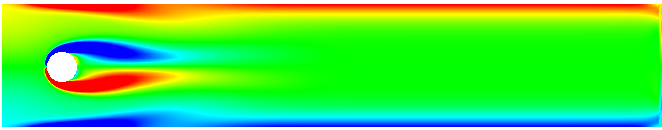
\includegraphics[width=0.8\textwidth]{png/cy-2.png}

    \vspace{.9em}

    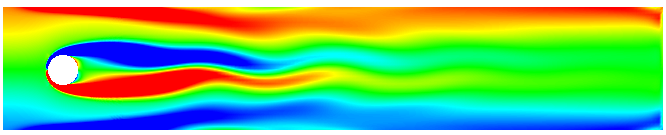
\includegraphics[width=0.8\textwidth]{png/cy-4.png}

    \vspace{.8em}

    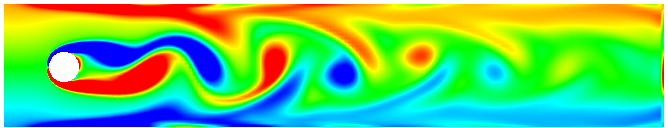
\includegraphics[width=0.8\textwidth]{png/cy-5.png}

    \vspace{.8em}

    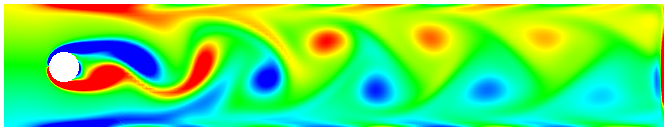
\includegraphics[width=0.8\textwidth]{png/cy-6.png}

    \vspace{.8em}

    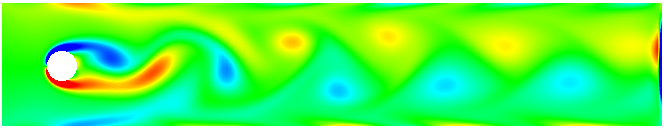
\includegraphics[width=0.8\textwidth]{png/cy-7.png}

    \vspace{.8em}

    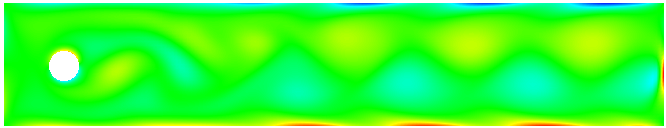
\includegraphics[width=0.8\textwidth]{png/cy-8.png}
    \caption{Vortricity plots of the cylindrical turbulence test. 
             $t=[2,4,5,6,7,8]$.}
\end{figure}

\subsubsection{Lip-driven cavity}

For the \textbf{lip-driven cavity} test, we set the condition at
the top boundary $y=1$ to be $\mathbf{u}=(1,0)$. Other boundaries
are set to be no-slip. The numerical test is running on a uniform grid 
with $h=\frac{1}{128}$. We set the time step $k=0.002$. The results
are shown in Fig. 4.

\begin{figure}[H]
    \centering
    \begin{minipage}[t]{0.45\linewidth}
        \centering
        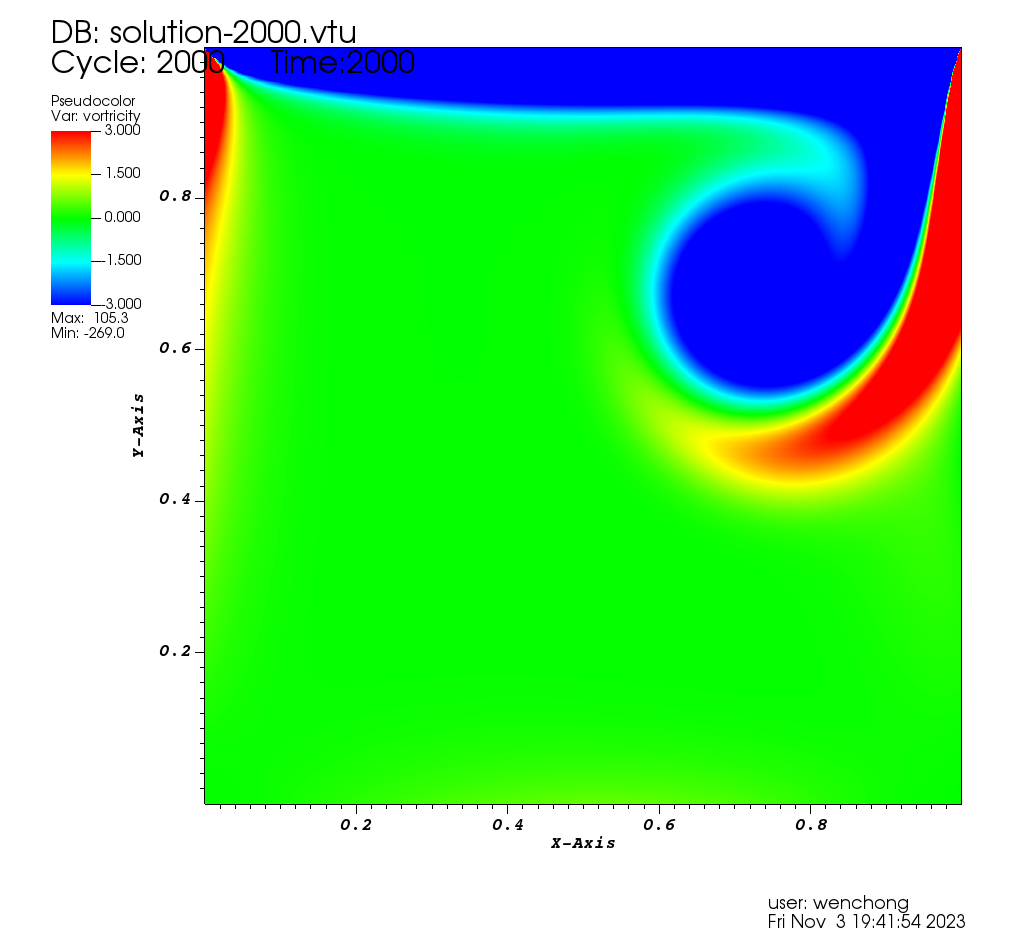
\includegraphics[width=0.9\linewidth]{png/lip-4.png}
        \caption*{(a) $t=4$.}
        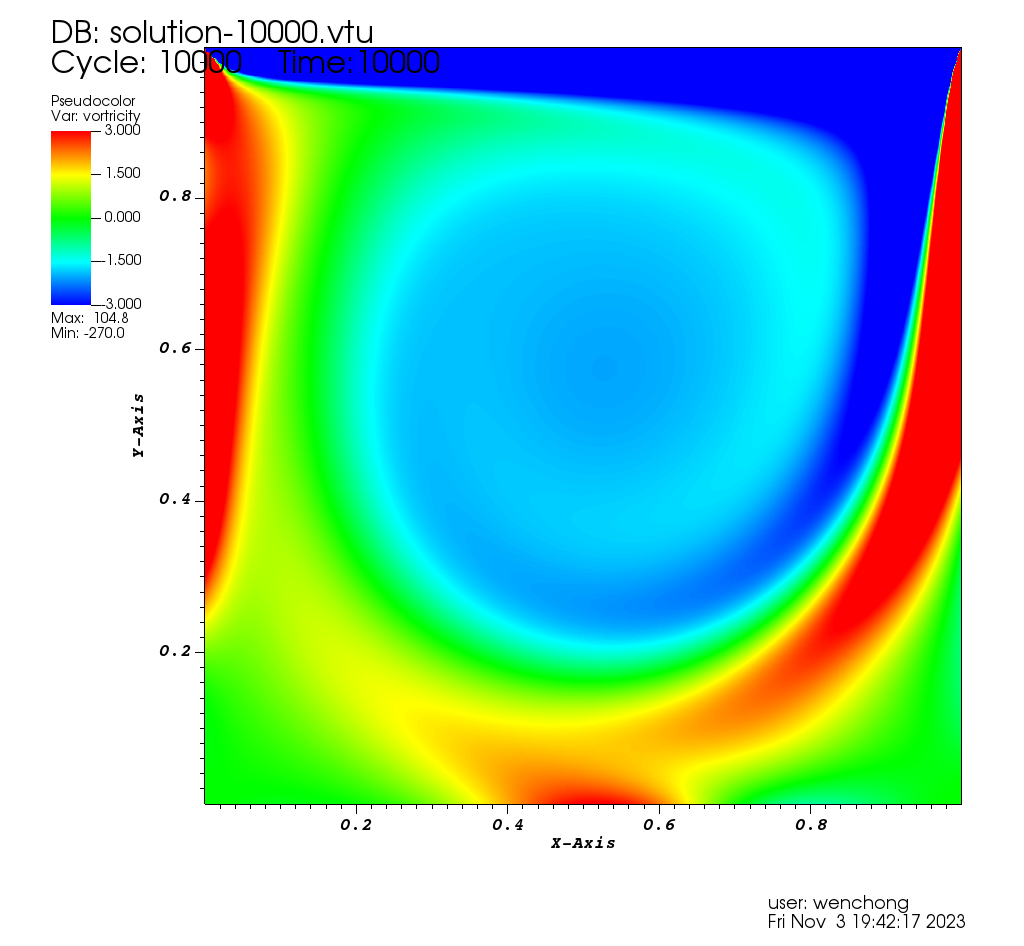
\includegraphics[width=0.9\linewidth]{png/lip-20.png}
        \caption*{(c) $t=20$.}
    \end{minipage}
    \begin{minipage}[t]{0.45\linewidth}
        \centering
        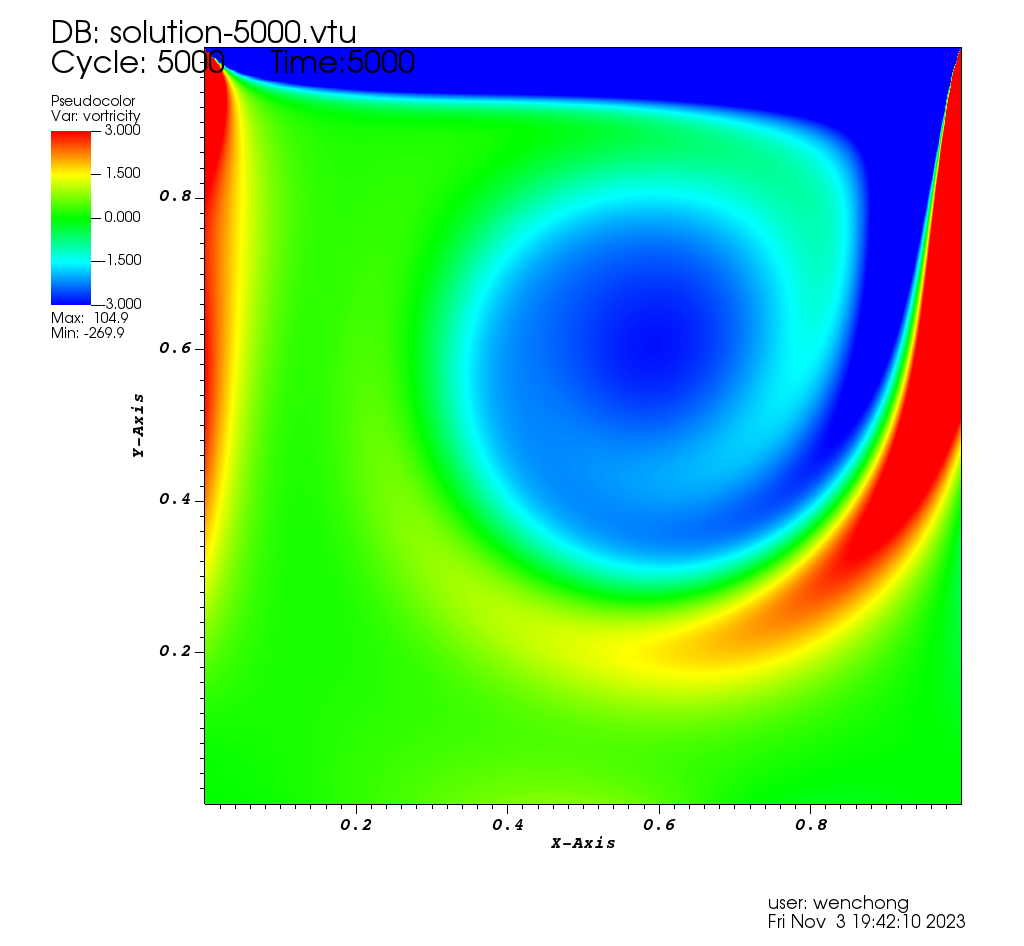
\includegraphics[width=0.9\linewidth]{png/lip-10.png}
        \caption*{(b) $t=10$.}
        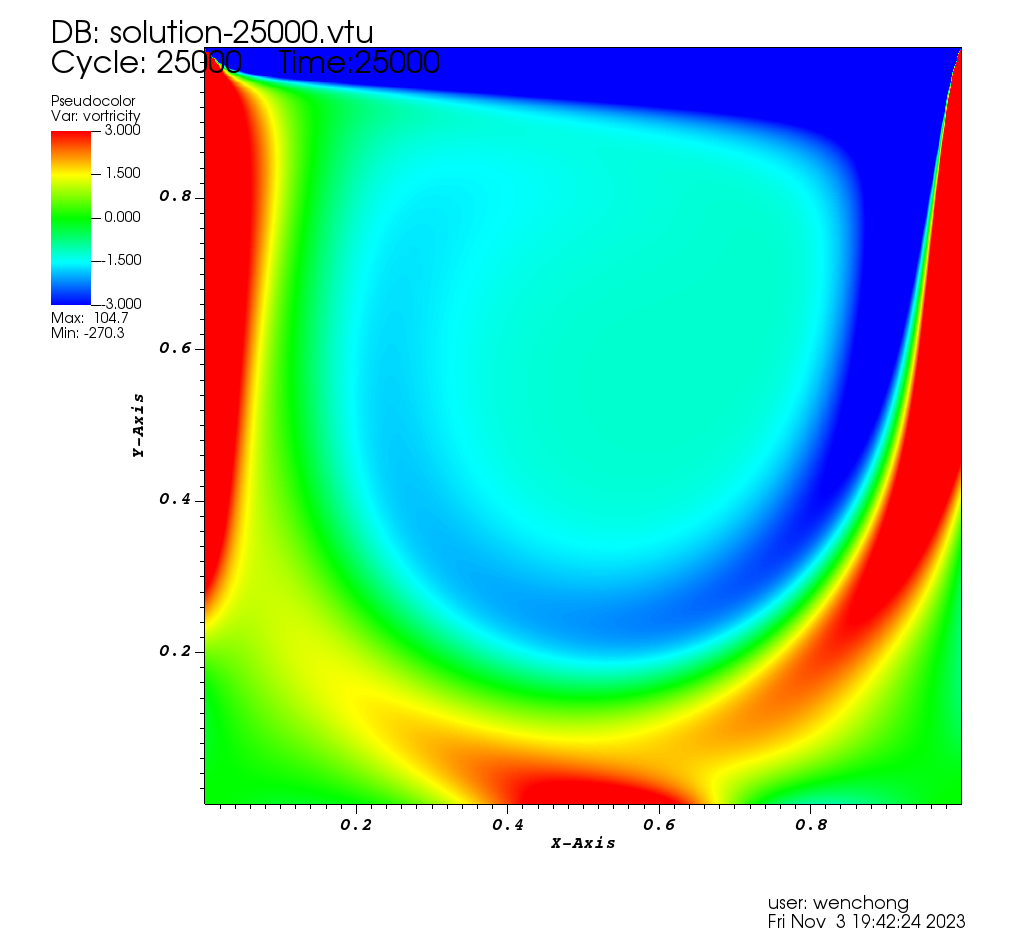
\includegraphics[width=0.9\linewidth]{png/lip-50.png}
        \caption*{(d) $t=50$.}
    \end{minipage}
    \caption{Vortricity plots of the lip-driven cavity test.}
\end{figure}

\section{Future work}

In my graduation thesis, things I want to do are listed below.

\begin{enumerate}
    \item A solver to the INSE with GePUP, see \cite{Zhang2016}.
    \item A solver to the Boussinesq equations.
    \item Extend all finished works to 3D.
    \item Supplement relative theoretical analysis.
\end{enumerate}

In the future, I want to learn DG methods. And implement the GePUP with
DG methods.

\printbibliography[heading=bibintoc,title=\ebibname]

\appendix
%\appendixpage
\addappheadtotoc

\end{document}
